\section{Parallel Execution of Test Suites}
\label{sec:modes}

\Mar{add a sentence to introduce this section at a higher abstraction
  level.}  Parallelism in test execution can be obtained at different
levels.  Figure~\ref{fig:levels} illustrates some of these levels.

This paper focuses at lower-level parallelism, obtained with parallel
computation at CPUs and threads in a given machine.  This kind of
parallelism is enabled through build systems and testing frameworks.
Given the proliferation of multicore machines it is not surprising
that testing frameworks provide today support for parallel test
execution with the goal of running tests more
efficiently~\cite{junit-org,testng,nunit}.  Build systems wrap
parallel features offered by testing frameworks to facilitate the use
of such technology\cite{maven-surefire-plugin}.  In the following we
elaborate relevant features of these components focusing on Java,
Maven, and JUnit but the discussion can be generalized to other
languages, build systems, and testing frameworks.

Note that lower-level parallelism is a complement to higher-level
parallelism that could be enabled through server farms.  For the
scenario of large IT organizations, lower-level parallelization
schemes could leverage the computing power of server nodes in addition
to the aggregate processing power of the farm.  Lower-level
parallelism fits particularly well smaller organizations (/projects)
with relatively high testing costs but lower budgets.
\Comment{
    Unfortunately, these solutions can't be used out-of-the-box:
    unrestricted parallel execution of tests can produce
    non-deterministic results as developers typically do not provision
    protection to concurrent accesses originated from arbitrary program
    points (\ie{}, tests).  We refer to this problem as Parallel
    Execution Flakiness (\pef{}).

    %% These solutions enable the
    %% use of commodity hardware to maximize CPU usage\footnote{In the case
    %%   of the Java language, for example, it is possible to explore
    %%   parallelism across and within JVMs.}.  

    To illustrate the importance of parallel test execution and
    the problem of \pef{} let's consider the case of the ``core'' module
    from the Apache Camel project~\cite{apache-camel-web}.  This module
    contains 5,679 test cases, declared in 2,356 test classes.  We ran
    those tests in a machine with 16GB of memory and 8 virtual CPUs (4
    cores with 2 native threads each).  Sequential test execution takes
    24m50s to run this test set.  Execution of the same test set takes
    2m28s when we configured parallel execution to fork a JVM per CPU and
    execute test classes, uniquely allocated to that JVM, sequentially but
    running test methods from each class in separate threads.  Note that
    this is an order of magnitude speedup (10.07x)\Fix{Need to understand
    why this is 10x as opposed to something closer to 7x - I didn't get
    your concern here}.  Unfortunately, due to \pef{}, $\sim$2\% (114 of
    5,679) of the tests fail when executed in parallel.  It is important
    to notice that the ratio of failures varies with the project as it
    depends on factors such as length of test cases and amount of shared
    state across tests.

    \pef{} is an important obstacle to enable parallel test execution.
    Conceptually, higher parallelization can result in higher chances of
    concurrency-related problems.  It is important to execute tests
    efficiently without sacrificing reliability
    \Fix{gap between pars?? What gap?}
}

\subsection{Testing Framework}

The list below shortly describes the choices to control parallelism
within a JVM.

\begin{figure}[t!]
  \centering
  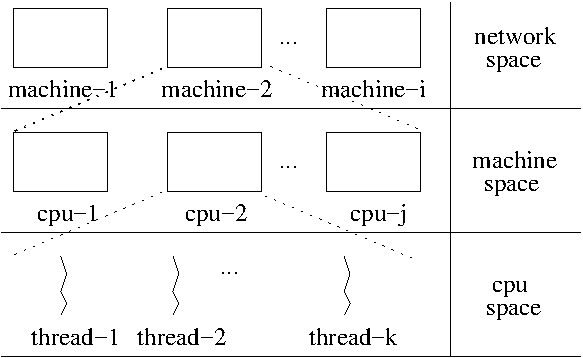
\includegraphics[width=0.4\textwidth]{figs/parallel-levels.pdf}
  \caption{\label{fig:levels}Levels of parallelism.}
\end{figure}

\newcommand{\Seq}{L0}
\newcommand{\ParClassSeqMeth}{L1}
\newcommand{\SeqClassParMeth}{L2}
\newcommand{\ParClassParMeth}{L3}

\begin{itemize}
\item \textbf{Sequential (\Seq).}~This configuration results in
    sequential execution of test classes and their methods, according
    to a given order defined in the testing framework (\eg, the order
    of methods returned by Java Reflection
    API)~\cite{junit-test-order}. For JUnit, this is the default
    configuration.

\item \textbf{Sequential classes; parallel methods
  (\ParClassSeqMeth{}).} This configuration results in the sequential
  execution of the test classes assigned to the JVM.  However, within
  each class, test methods run in parallel. In JUnit,
  \emph{ParallelComputer} provides support to parallel execution; it
  instantiates a test runner with a \emph{ExecutorService} from the
  Java Concurrent API. Each test method is executed in a separated
  thread as the thread pool creates new threads on-demand and reuse
  them if any thread is available.

\Comment{http://junit.org/junit4/javadoc/latest/src-html/org/junit/experimental/ParallelComputer.html#line.14}

\item \textbf{Parallel classes; sequential methods
  (\SeqClassParMeth{}).}  This configuration results in the parallel
  execution of test classes but test methods of any given class are
  executed sequentially. As in \ParClassSeqMeth, the runner has a
  cached thread poll. However, instead of executing test methods from
  a single test class, the test suite runner executes classes in
  separated threads and methods in sequence within each thread.

\item \textbf{Parallel methods (\ParClassParMeth).} This configuration
  results in parallel execution of any given test method of any class.
  \Jbc{I need to confirm this but AFAIK this is how it happens}
  It is the union of \ParClassSeqMeth and \SeqClassParMeth: there is a
  thread pool for execution classes on separated threads and within
  each test class, there is a runner with a \emph{ExecutorService} to
  run test methods in parallel.
\end{itemize}

\Jbc{I have to understand better how Surefire executes tests. I'm
afraid it has its own wrapper classes and reuse JUnit core
functionalities. I'm saying this because JUnit does not offer a finer
control over thread numbers while this configuration is possible with
Surefire} For example, Figure~\ref{fig:surefire} illustrates how to
configure Maven to execute classes sequentially (default behavior) and
test methods in parallel. Although this configuration is defined in
the build file (\eg, \emph{pom.xml} on Maven), \Fix{these settings are
forwarded to the underlying testing framework (\eg, JUnit). In case of
JUnit,}

\begin{figure}[h!]
    \centering
    \lstset{language=XML}
    \begin{lstlisting}
    <plugin>
        <groupId>org.apache.maven.plugins</groupId>
        <artifactId>maven-surefire-plugin</artifactId>
        <configuration>
            <parallel>methods</parallel>
            <threadCount>2</threadCount>
            <perCoreThreadCount>true</perCoreThreadCount>
        </configuration>
    </plugin>
    \end{lstlisting}
    \caption{\label{fig:surefire}\Fix{...}}
\end{figure}

\Fix{We need a par. providing rationale in to explain (points in
favor/against) these choices.}

\subsection{Build Systems}
Build systems, such as Maven\footnote{\url{maven.apache.org}},
typically provide the option to \emph{fork} JVM instances
proportionally to available cores in the machine.  If the option
``fork JVM'' is enabled, Maven will allocate a user-provided number of
JVM instances to each core in the machine and will allocate each test
class to exactly one JVM.  Note that there is no guarantee to
uniformly distribute load to each JVM given that the build system uses
classes as the unit to specify test tasks.\Fix{we need to know how
Maven allocates test classes to JVMs}
